% planisphere.tex
%
% The LaTeX code in this file brings together into a single document the
% various components of the model planisphere.
%
% Copyright (C) 2014-2019 Dominic Ford <dcf21-www@dcford.org.uk>
%
% This code is free software; you can redistribute it and/or modify it under
% the terms of the GNU General Public License as published by the Free Software
% Foundation; either version 2 of the License, or (at your option) any later
% version.
%
% You should have received a copy of the GNU General Public License along with
% this file; if not, write to the Free Software Foundation, Inc., 51 Franklin
% Street, Fifth Floor, Boston, MA  02110-1301, USA

% ----------------------------------------------------------------------------

\documentclass[a4paper,onecolumn,10pt]{article}
\usepackage[dvips]{graphicx}
\usepackage{fancyhdr,url}
\usepackage[utf8]{inputenc}
\usepackage{parskip}
\usepackage[pdftitle={Crie seu próprio planisfério}, pdfauthor={Dominic Ford}, pdfsubject={Crie seu próprio planisfério}, pdfkeywords={Crie seu próprio planisfério}, colorlinks=true, linkcolor=blue, citecolor=blue, filecolor=blue, urlcolor=blue]{hyperref}
\usepackage[T1]{fontenc}
\renewcommand{\familydefault}{\sfdefault}
\pagestyle{fancy}

\lhead{\it FAÇA SEU PRÓPRIO PLANISFÉRIO}
\chead{}
\rhead{\thepage}
\lfoot{}\rfoot{}
\cfoot{\bf\footnotesize\copyright\ 2014--2019 Dominic Ford. Distribuído sob o GNU General Public License, versão 3. Documento baixado de \url{https://in-the-sky.org/planisphere/}}

\fancypagestyle{plain}{%
\fancyhf{} % clear all header and footer fields
\renewcommand{\headrulewidth}{0pt}
\renewcommand{\footrulewidth}{0pt}}

\title{Faça seu próprio planisfério}
\author{Dominic Ford}
\date{2014--2019}

\begin{document}
\maketitle
\setcounter{footnote}{1}

Um planisfério é um dispositivo portátil simples que mostra um mapa de quais estrelas 
são visíveis no céu noturno a qualquer momento. Ao girar uma roda, ele mostra
como as estrelas se movem pelo céu durante a noite e quão diferentes
constelações são visíveis em diferentes épocas do ano.

Apresento aqui um kit que você pode baixar e imprimir para criar o seu próprio
planisfério sem papel ou papelão.

O design de um planisfério depende da localização geográfica em que deve
ser usado, pois estrelas diferentes são visíveis de lugares diferentes. eu tenho
criou kits para uso em uma grande variedade de latitudes, que você pode baixar em

\url{https://in-the-sky.org/planisphere/}

O planisfério apresentado neste documento foi projetado para uso a uma latitude de
\input{tmp/lat}.
 
\section*{O que você precisa}

\begin{itemize}
\item Duas folhas de papel A4 ou, de preferência, cartão fino.
\item Tesoura.
\item Um prendedor de pinos divididos.
\item Opcional: uma folha de plástico transparente, p. acetato projetado para uso 
com projetores aéreos.
\item Opcional: Um pouco de cola.
\end{itemize}

\section*{Instruções de montagem}

{\bf Passo 1} -- Os planisférios parecem um pouco diferentes dependendo de onde você 
viver. O planisfério preparado neste documento foi projetado para uso em qualquer 
lugar da Terra que está a alguns graus de latitude \input{tmp/lat}. Se você vive
em outro lugar, você deve baixar um kit alternativo de

\url{https://in-the-sky.org/planisphere/}

{\bf Passo 2} -- Imprima as páginas na parte de trás deste arquivo PDF, mostrando o
roda estelar e o corpo do planisfério, em duas folhas de papel separadas,
ou mais preferencialmente em cartão fino.

{\bf Passo 3} -- Corte cuidadosamente a roda estelar e o corpo do
planisfério. Corte também a área cinza sombreada do corpo do planisfério e
se você tiver, a grade de linhas que você imprimiu em transparentes
plástico. Se você estiver usando papelão, poderá marcar cuidadosamente o corpo
do planisfério ao longo da linha pontilhada para facilitar a dobra
esta linha mais tarde.

{\bf Passo 4} -- A roda estelar tem um pequeno círculo no centro e a
O corpo do planisfério possui um pequeno círculo correspondente na parte inferior. 
Faça um pequeno buraco (cerca de 2 mm de diâmetro) em cada um. Se houver uma broca 
de papel à mão, estas são ideais, caso contrário, use um ponto de bússola e 
amplie o furo girando em uma circular movimento.

{\bf Step 5} -- Coloque um prendedor de pino dividido no meio da
estrela, com a cabeça do fixador contra o lado impresso do roda estelar. 
Em seguida, encaixe o corpo do planisfério no mesmo fixador, com o lado 
impresso voltado para a parte traseira do fixador. Dobre o prendedor para 
baixo prenda as duas folhas de papelão juntas.

{\bf Passo 6 (Opcional)} -- Se você imprimiu a página final do arquivo PDF
em uma folha de plástico, agora você deve colar esta grade de linhas sobre o
janela de visualização cortada do corpo do planisfério.

{\bf Passo 7} -- Dobre o corpo do planisfério ao longo da linha pontilhada, 
de modo que a frente da roda estrelada apareça pela janela que você cortou
o corpo.

{\bf Parabéns, seu planisfério está pronto para uso!}

\section*{Como usar seu planisfério}

Gire a roda estelar até encontrar o ponto em sua borda onde a data de hoje
está marcado e alinhe esse ponto com a hora atual. A janela de visualização agora
mostra todas as constelações que são visíveis no céu.

Vá para fora e enfrente o norte. Segurando o planisfério no céu, as estrelas
marcado na parte inferior da janela de visualização deve corresponder àqueles que 
você veja no céu na sua frente.

Vire para o leste ou oeste e gire o planisfério para que a palavra "Leste"
ou "Oeste" está na parte inferior da janela. Mais uma vez, as estrelas no fundo
da janela de visualização deve coincidir com aqueles que você vê no céu em
na sua frente.

Se você imprimiu a grade de altitude e linhas de azimute em plástico transparente,
essas linhas permitem descobrir como os objetos altos aparecerão no céu e em
qual direção. Os círculos são desenhados em altitudes de 10, 20, 30, ..., 80
graus acima do horizonte. Para referência, uma distância de dez graus aproximadamente
equivale a uma extensão de mão no comprimento do braço. As linhas curvas são linhas 
verticais pontos de conexão no horizonte até o ponto imediatamente acima da cabeça.
Eles são desenhados nas direções cardinais S, SSE, SE, ESE, E, etc.

\section*{Planisférios personalizados}

Este kit planisphere foi projetado usando uma coleção de scripts Python e o
biblioteca de gráficos pycairo. Se você deseja personalizar seu planisfério,
seja bem-vindo ao baixar os scripts da minha conta do GitHub e modificá-los,
fornecendo o crédito da fonte:

\url{https://github.com/dcf21/planisphere}

\section*{License}

Como tudo no {\tt In-The-Sky.org}, esses kits do planisfério são
\copyright\ Dominic Ford. No entanto, tudo no {\tt In-The-Sky.org} é
fornecido para o benefício de astrônomos amadores em todo o mundo, e você é bem-vindo
modificar e/ou redistribuir qualquer material deste site, sob o
seguintes condições: (1) Qualquer item que tenha um texto de direitos autorais associado {\bf
deve} incluir o texto {\bf não modificado} na sua versão redistribuída, (2) Você
{\bf} devo me creditar, Dominic Ford, como autor original e direitos autorais
(3) Você {\bf} não poderá obter nenhum lucro com a reprodução de
material deste site, {\bf a menos que você seja uma instituição de caridade registrada cuja
objetivo expresso é o avanço da ciência astronômica, {\bf ou} você ter a
permissão por escrito do autor.

\newpage

\centerline{\includegraphics{tmp/starwheel}}

\vspace{1cm}
A roda estelar central do planisfério, que deve ser encaixada dentro do suporte dobrado.

\newpage
\thispagestyle{empty}
\vspace*{-3.0cm}
\centerline{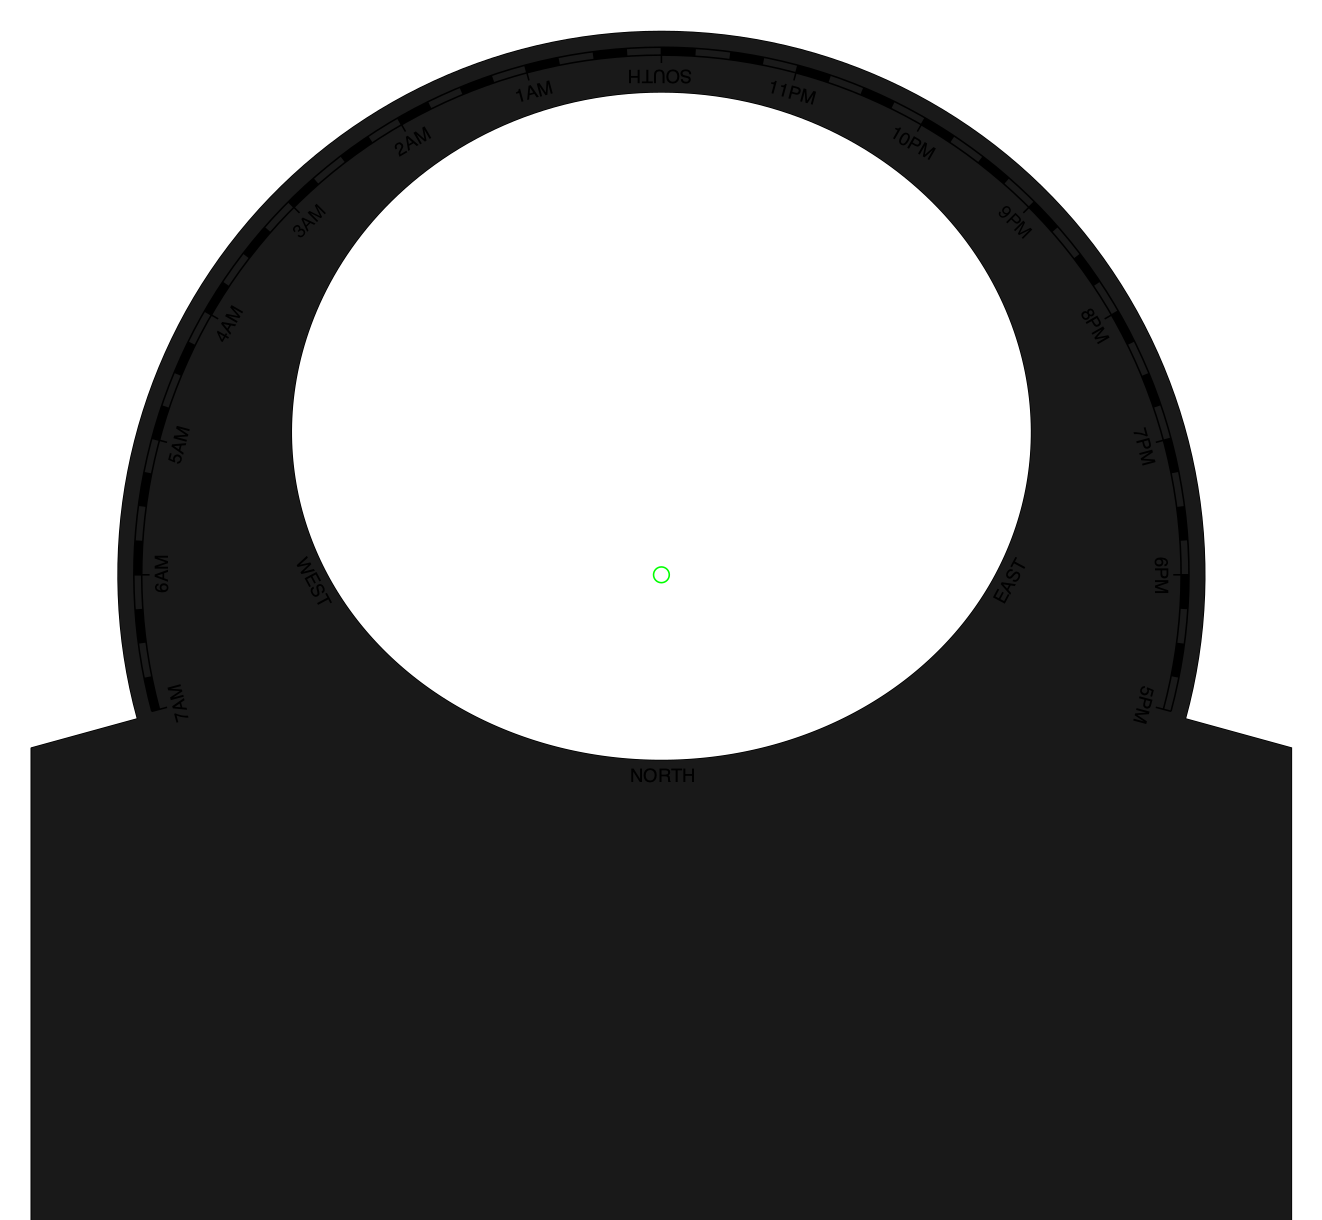
\includegraphics{tmp/holder}}
\newpage

\centerline{\includegraphics{tmp/altaz}}

\vspace{1cm}
Essa grade de linhas pode opcionalmente ser impressa em plástico transparente e colada na janela recortada no corpo do planisfério para mostrar as altitudes dos objetos no céu e suas direções.

\end{document}

